\documentclass[1p]{elsarticle_modified}
%\bibliographystyle{elsarticle-num}

%\usepackage[colorlinks]{hyperref}
%\usepackage{abbrmath_seonhwa} %\Abb, \Ascr, \Acal ,\Abf, \Afrak
\usepackage{amsfonts}
\usepackage{amssymb}
\usepackage{amsmath}
\usepackage{amsthm}
\usepackage{scalefnt}
\usepackage{amsbsy}
\usepackage{kotex}
\usepackage{caption}
\usepackage{subfig}
\usepackage{color}
\usepackage{graphicx}
\usepackage{xcolor} %% white, black, red, green, blue, cyan, magenta, yellow
\usepackage{float}
\usepackage{setspace}
\usepackage{hyperref}

\usepackage{tikz}
\usetikzlibrary{arrows}

\usepackage{multirow}
\usepackage{array} % fixed length table
\usepackage{hhline}

%%%%%%%%%%%%%%%%%%%%%
\makeatletter
\renewcommand*\env@matrix[1][\arraystretch]{%
	\edef\arraystretch{#1}%
	\hskip -\arraycolsep
	\let\@ifnextchar\new@ifnextchar
	\array{*\c@MaxMatrixCols c}}
\makeatother %https://tex.stackexchange.com/questions/14071/how-can-i-increase-the-line-spacing-in-a-matrix
%%%%%%%%%%%%%%%

\usepackage[normalem]{ulem}

\newcommand{\msout}[1]{\ifmmode\text{\sout{\ensuremath{#1}}}\else\sout{#1}\fi}
%SOURCE: \msout is \stkout macro in https://tex.stackexchange.com/questions/20609/strikeout-in-math-mode

\newcommand{\cancel}[1]{
	\ifmmode
	{\color{red}\msout{#1}}
	\else
	{\color{red}\sout{#1}}
	\fi
}

\newcommand{\add}[1]{
	{\color{blue}\uwave{#1}}
}

\newcommand{\replace}[2]{
	\ifmmode
	{\color{red}\msout{#1}}{\color{blue}\uwave{#2}}
	\else
	{\color{red}\sout{#1}}{\color{blue}\uwave{#2}}
	\fi
}

\newcommand{\Sol}{\mathcal{S}} %segment
\newcommand{\D}{D} %diagram
\newcommand{\A}{\mathcal{A}} %arc


%%%%%%%%%%%%%%%%%%%%%%%%%%%%%5 test

\def\sl{\operatorname{\textup{SL}}(2,\Cbb)}
\def\psl{\operatorname{\textup{PSL}}(2,\Cbb)}
\def\quan{\mkern 1mu \triangleright \mkern 1mu}

\theoremstyle{definition}
\newtheorem{thm}{Theorem}[section]
\newtheorem{prop}[thm]{Proposition}
\newtheorem{lem}[thm]{Lemma}
\newtheorem{ques}[thm]{Question}
\newtheorem{cor}[thm]{Corollary}
\newtheorem{defn}[thm]{Definition}
\newtheorem{exam}[thm]{Example}
\newtheorem{rmk}[thm]{Remark}
\newtheorem{alg}[thm]{Algorithm}

\newcommand{\I}{\sqrt{-1}}
\begin{document}

%\begin{frontmatter}
%
%\title{Boundary parabolic representations of knots up to 8 crossings}
%
%%% Group authors per affiliation:
%\author{Yunhi Cho} 
%\address{Department of Mathematics, University of Seoul, Seoul, Korea}
%\ead{yhcho@uos.ac.kr}
%
%
%\author{Seonhwa Kim} %\fnref{s_kim}}
%\address{Center for Geometry and Physics, Institute for Basic Science, Pohang, 37673, Korea}
%\ead{ryeona17@ibs.re.kr}
%
%\author{Hyuk Kim}
%\address{Department of Mathematical Sciences, Seoul National University, Seoul 08826, Korea}
%\ead{hyukkim@snu.ac.kr}
%
%\author{Seokbeom Yoon}
%\address{Department of Mathematical Sciences, Seoul National University, Seoul, 08826,  Korea}
%\ead{sbyoon15@snu.ac.kr}
%
%\begin{abstract}
%We find all boundary parabolic representation of knots up to 8 crossings.
%
%\end{abstract}
%\begin{keyword}
%    \MSC[2010] 57M25 
%\end{keyword}
%
%\end{frontmatter}

%\linenumbers
%\tableofcontents
%
\newcommand\colored[1]{\textcolor{white}{\rule[-0.35ex]{0.8em}{1.4ex}}\kern-0.8em\color{red} #1}%
%\newcommand\colored[1]{\textcolor{white}{ #1}\kern-2.17ex	\textcolor{white}{ #1}\kern-1.81ex	\textcolor{white}{ #1}\kern-2.15ex\color{red}#1	}

{\Large $\underline{12n_{0047}~(K12n_{0047})}$}

\setlength{\tabcolsep}{10pt}
\renewcommand{\arraystretch}{1.6}
\vspace{1cm}\begin{tabular}{m{100pt}>{\centering\arraybackslash}m{274pt}}
\multirow{5}{120pt}{
	\centering
	\includegraphics[width=112pt]{../../../GIT/diagram.site/Diagrams/png/2136_12n_0047.png}\\
\ \ \ A knot diagram\footnotemark}&
\allowdisplaybreaks
\textbf{Linearized knot diagam} \\
\cline{2-2}
 &
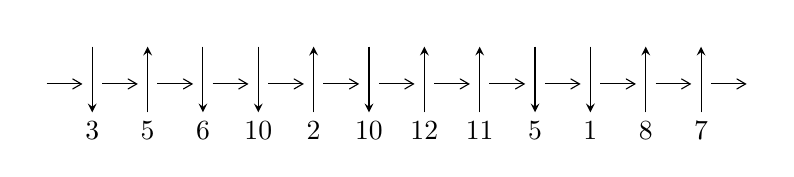
\begin{tikzpicture}[x=20pt, y=17pt]
	% nodes
	\node (C0) at (0, 0) {};
	\node (C1) at (1, 0) {};
	\node (C1U) at (1, +1) {};
	\node (C1D) at (1, -1) {3};

	\node (C2) at (2, 0) {};
	\node (C2U) at (2, +1) {};
	\node (C2D) at (2, -1) {5};

	\node (C3) at (3, 0) {};
	\node (C3U) at (3, +1) {};
	\node (C3D) at (3, -1) {6};

	\node (C4) at (4, 0) {};
	\node (C4U) at (4, +1) {};
	\node (C4D) at (4, -1) {10};

	\node (C5) at (5, 0) {};
	\node (C5U) at (5, +1) {};
	\node (C5D) at (5, -1) {2};

	\node (C6) at (6, 0) {};
	\node (C6U) at (6, +1) {};
	\node (C6D) at (6, -1) {10};

	\node (C7) at (7, 0) {};
	\node (C7U) at (7, +1) {};
	\node (C7D) at (7, -1) {12};

	\node (C8) at (8, 0) {};
	\node (C8U) at (8, +1) {};
	\node (C8D) at (8, -1) {11};

	\node (C9) at (9, 0) {};
	\node (C9U) at (9, +1) {};
	\node (C9D) at (9, -1) {5};

	\node (C10) at (10, 0) {};
	\node (C10U) at (10, +1) {};
	\node (C10D) at (10, -1) {1};

	\node (C11) at (11, 0) {};
	\node (C11U) at (11, +1) {};
	\node (C11D) at (11, -1) {8};

	\node (C12) at (12, 0) {};
	\node (C12U) at (12, +1) {};
	\node (C12D) at (12, -1) {7};
	\node (C13) at (13, 0) {};

	% arrows
	\draw[->,>={angle 60}]
	(C0) edge (C1) (C1) edge (C2) (C2) edge (C3) (C3) edge (C4) (C4) edge (C5) (C5) edge (C6) (C6) edge (C7) (C7) edge (C8) (C8) edge (C9) (C9) edge (C10) (C10) edge (C11) (C11) edge (C12) (C12) edge (C13) ;	\draw[->,>=stealth]
	(C1U) edge (C1D) (C2D) edge (C2U) (C3U) edge (C3D) (C4U) edge (C4D) (C5D) edge (C5U) (C6U) edge (C6D) (C7D) edge (C7U) (C8D) edge (C8U) (C9U) edge (C9D) (C10U) edge (C10D) (C11D) edge (C11U) (C12D) edge (C12U) ;
	\end{tikzpicture} \\
\hhline{~~} \\& 
\textbf{Solving Sequence} \\ \cline{2-2} 
 &
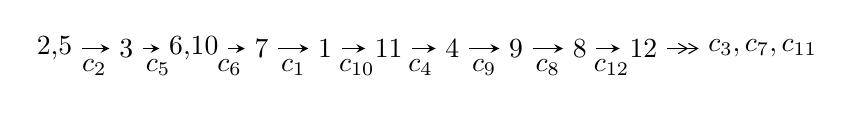
\begin{tikzpicture}[x=23pt, y=7pt]
	% node
	\node (A0) at (-1/8, 0) {2,5};
	\node (A1) at (1, 0) {3};
	\node (A2) at (33/16, 0) {6,10};
	\node (A3) at (25/8, 0) {7};
	\node (A4) at (33/8, 0) {1};
	\node (A5) at (41/8, 0) {11};
	\node (A6) at (49/8, 0) {4};
	\node (A7) at (57/8, 0) {9};
	\node (A8) at (65/8, 0) {8};
	\node (A9) at (73/8, 0) {12};
	\node (C1) at (1/2, -1) {$c_{2}$};
	\node (C2) at (3/2, -1) {$c_{5}$};
	\node (C3) at (21/8, -1) {$c_{6}$};
	\node (C4) at (29/8, -1) {$c_{1}$};
	\node (C5) at (37/8, -1) {$c_{10}$};
	\node (C6) at (45/8, -1) {$c_{4}$};
	\node (C7) at (53/8, -1) {$c_{9}$};
	\node (C8) at (61/8, -1) {$c_{8}$};
	\node (C9) at (69/8, -1) {$c_{12}$};
	\node (A10) at (11, 0) {$c_{3},c_{7},c_{11}$};

	% edge
	\draw[->,>=stealth]	
	(A0) edge (A1) (A1) edge (A2) (A2) edge (A3) (A3) edge (A4) (A4) edge (A5) (A5) edge (A6) (A6) edge (A7) (A7) edge (A8) (A8) edge (A9) ;
	\draw[->>,>={angle 60}]	
	(A9) edge (A10);
\end{tikzpicture} \\ 

\end{tabular} \\

\footnotetext{
The image of knot diagram is generated by the software ``\textbf{Draw programme}" developed by Andrew Bartholomew(\url{http://www.layer8.co.uk/maths/draw/index.htm\#Running-draw}), where we modified some parts for our purpose(\url{https://github.com/CATsTAILs/LinksPainter}).
}\phantom \\ \newline 
\centering \textbf{Ideals for irreducible components\footnotemark of $X_{\text{par}}$} 
 
\begin{align*}
I^u_{1}&=\langle 
-8 u^{36}+17 u^{35}+\cdots+8 b+21,\;-7 u^{36}+31 u^{35}+\cdots+4 a+11,\;u^{37}-5 u^{36}+\cdots+u-1\rangle \\
I^u_{2}&=\langle 
b^4- b^3 u- b^3+b^2 u- u-1,\;a,\;u^2+u+1\rangle \\
\\
\end{align*}
\raggedright * 2 irreducible components of $\dim_{\mathbb{C}}=0$, with total 45 representations.\\
\footnotetext{All coefficients of polynomials are rational numbers. But the coefficients are sometimes approximated in decimal forms when there is not enough margin.}
\newpage
\renewcommand{\arraystretch}{1}
\centering \section*{I. $I^u_{1}= \langle -8 u^{36}+17 u^{35}+\cdots+8 b+21,\;-7 u^{36}+31 u^{35}+\cdots+4 a+11,\;u^{37}-5 u^{36}+\cdots+u-1 \rangle$}
\flushleft \textbf{(i) Arc colorings}\\
\begin{tabular}{m{7pt} m{180pt} m{7pt} m{180pt} }
\flushright $a_{2}=$&$\begin{pmatrix}1\\0\end{pmatrix}$ \\
\flushright $a_{5}=$&$\begin{pmatrix}0\\u\end{pmatrix}$ \\
\flushright $a_{3}=$&$\begin{pmatrix}1\\- u^2\end{pmatrix}$ \\
\flushright $a_{6}=$&$\begin{pmatrix}u\\u\end{pmatrix}$ \\
\flushright $a_{10}=$&$\begin{pmatrix}\frac{7}{4} u^{36}-\frac{31}{4} u^{35}+\cdots+\frac{7}{4} u-\frac{11}{4}\\u^{36}-\frac{17}{8} u^{35}+\cdots+\frac{7}{2} u-\frac{21}{8}\end{pmatrix}$ \\
\flushright $a_{7}=$&$\begin{pmatrix}- u^2-1\\-\frac{1}{8} u^{36}+\frac{5}{8} u^{35}+\cdots+\frac{17}{8} u-\frac{1}{8}\end{pmatrix}$ \\
\flushright $a_{1}=$&$\begin{pmatrix}u^2+1\\- u^4\end{pmatrix}$ \\
\flushright $a_{11}=$&$\begin{pmatrix}\frac{15}{8} u^{36}-\frac{67}{8} u^{35}+\cdots+\frac{3}{8} u-\frac{13}{8}\\\frac{1}{8} u^{36}+\frac{5}{4} u^{35}+\cdots+\frac{33}{8} u-\frac{7}{2}\end{pmatrix}$ \\
\flushright $a_{4}=$&$\begin{pmatrix}u^4+u^2+1\\u^4\end{pmatrix}$ \\
\flushright $a_{9}=$&$\begin{pmatrix}\frac{7}{4} u^{36}-\frac{31}{4} u^{35}+\cdots+\frac{7}{4} u-\frac{11}{4}\\\frac{11}{4} u^{36}-\frac{69}{8} u^{35}+\cdots+\frac{11}{4} u-\frac{29}{8}\end{pmatrix}$ \\
\flushright $a_{8}=$&$\begin{pmatrix}\frac{5}{4} u^{36}-\frac{11}{2} u^{35}+\cdots+\frac{1}{2} u-\frac{3}{4}\\-\frac{3}{4} u^{36}+\frac{61}{8} u^{35}+\cdots+\frac{19}{4} u-\frac{45}{8}\end{pmatrix}$ \\
\flushright $a_{12}=$&$\begin{pmatrix}-\frac{1}{8} u^{36}+\frac{1}{2} u^{35}+\cdots-\frac{15}{8} u+1\\u^{36}-\frac{47}{8} u^{35}+\cdots-\frac{5}{4} u+\frac{15}{8}\end{pmatrix}$\\&\end{tabular}
\flushleft \textbf{(ii) Obstruction class $= -1$}\\~\\
\flushleft \textbf{(iii) Cusp Shapes $= -\frac{13}{8} u^{36}+10 u^{35}+\cdots+\frac{243}{8} u-\frac{13}{2}$}\\~\\
\newpage\renewcommand{\arraystretch}{1}
\flushleft \textbf{(iv) u-Polynomials at the component}\newline \\
\begin{tabular}{m{50pt}|m{274pt}}
Crossings & \hspace{64pt}u-Polynomials at each crossing \\
\hline $$\begin{aligned}c_{1}\end{aligned}$$&$\begin{aligned}
&u^{37}+23 u^{36}+\cdots-25 u-1
\end{aligned}$\\
\hline $$\begin{aligned}c_{2},c_{5}\end{aligned}$$&$\begin{aligned}
&u^{37}+5 u^{36}+\cdots+u+1
\end{aligned}$\\
\hline $$\begin{aligned}c_{3}\end{aligned}$$&$\begin{aligned}
&u^{37}-5 u^{36}+\cdots-7 u+1
\end{aligned}$\\
\hline $$\begin{aligned}c_{4},c_{9}\end{aligned}$$&$\begin{aligned}
&u^{37}- u^{36}+\cdots+384 u+256
\end{aligned}$\\
\hline $$\begin{aligned}c_{6}\end{aligned}$$&$\begin{aligned}
&u^{37}+3 u^{36}+\cdots- u+1
\end{aligned}$\\
\hline $$\begin{aligned}c_{7},c_{8},c_{11}\\c_{12}\end{aligned}$$&$\begin{aligned}
&u^{37}+3 u^{36}+\cdots+3 u+1
\end{aligned}$\\
\hline $$\begin{aligned}c_{10}\end{aligned}$$&$\begin{aligned}
&u^{37}-13 u^{36}+\cdots-2707 u-563
\end{aligned}$\\
\hline
\end{tabular}\\~\\
\newpage\renewcommand{\arraystretch}{1}
\flushleft \textbf{(v) Riley Polynomials at the component}\newline \\
\begin{tabular}{m{50pt}|m{274pt}}
Crossings & \hspace{64pt}Riley Polynomials at each crossing \\
\hline $$\begin{aligned}c_{1}\end{aligned}$$&$\begin{aligned}
&y^{37}-13 y^{36}+\cdots-101 y-1
\end{aligned}$\\
\hline $$\begin{aligned}c_{2},c_{5}\end{aligned}$$&$\begin{aligned}
&y^{37}+23 y^{36}+\cdots-25 y-1
\end{aligned}$\\
\hline $$\begin{aligned}c_{3}\end{aligned}$$&$\begin{aligned}
&y^{37}-49 y^{36}+\cdots-25 y-1
\end{aligned}$\\
\hline $$\begin{aligned}c_{4},c_{9}\end{aligned}$$&$\begin{aligned}
&y^{37}-45 y^{36}+\cdots+507904 y-65536
\end{aligned}$\\
\hline $$\begin{aligned}c_{6}\end{aligned}$$&$\begin{aligned}
&y^{37}-47 y^{36}+\cdots-21 y-1
\end{aligned}$\\
\hline $$\begin{aligned}c_{7},c_{8},c_{11}\\c_{12}\end{aligned}$$&$\begin{aligned}
&y^{37}+45 y^{36}+\cdots-21 y-1
\end{aligned}$\\
\hline $$\begin{aligned}c_{10}\end{aligned}$$&$\begin{aligned}
&y^{37}-27 y^{36}+\cdots+708095 y-316969
\end{aligned}$\\
\hline
\end{tabular}\\~\\
\newpage\flushleft \textbf{(vi) Complex Volumes and Cusp Shapes}
$$\begin{array}{c|c|c}  
\text{Solutions to }I^u_{1}& \I (\text{vol} + \sqrt{-1}CS) & \text{Cusp shape}\\
 \hline 
\begin{aligned}
u &= \phantom{-}0.974418 + 0.080590 I \\
a &= \phantom{-}1.70420 + 0.06611 I \\
b &= -0.049744 + 0.136325 I\end{aligned}
 & -6.68859 - 3.78454 I & -3.30270 + 3.82626 I \\ \hline\begin{aligned}
u &= \phantom{-}0.974418 - 0.080590 I \\
a &= \phantom{-}1.70420 - 0.06611 I \\
b &= -0.049744 - 0.136325 I\end{aligned}
 & -6.68859 + 3.78454 I & -3.30270 - 3.82626 I \\ \hline\begin{aligned}
u &= \phantom{-}0.231315 + 1.006220 I \\
a &= -0.542701 + 0.732426 I \\
b &= \phantom{-}0.34827 + 2.04966 I\end{aligned}
 & -8.03711 + 4.79124 I & -8.56176 - 2.65048 I \\ \hline\begin{aligned}
u &= \phantom{-}0.231315 - 1.006220 I \\
a &= -0.542701 - 0.732426 I \\
b &= \phantom{-}0.34827 - 2.04966 I\end{aligned}
 & -8.03711 - 4.79124 I & -8.56176 + 2.65048 I \\ \hline\begin{aligned}
u &= \phantom{-}1.028220 + 0.124183 I \\
a &= -1.74341 - 0.11482 I \\
b &= -0.037304 - 0.222366 I\end{aligned}
 & -15.2275 - 6.0970 I & -5.01510 + 2.60803 I \\ \hline\begin{aligned}
u &= \phantom{-}1.028220 - 0.124183 I \\
a &= -1.74341 + 0.11482 I \\
b &= -0.037304 + 0.222366 I\end{aligned}
 & -15.2275 + 6.0970 I & -5.01510 - 2.60803 I \\ \hline\begin{aligned}
u &= \phantom{-}0.136558 + 0.938853 I \\
a &= \phantom{-}0.637084 - 0.690045 I \\
b &= -0.37494 - 1.62263 I\end{aligned}
 & -0.94719 + 2.42286 I & -4.75761 - 3.49030 I \\ \hline\begin{aligned}
u &= \phantom{-}0.136558 - 0.938853 I \\
a &= \phantom{-}0.637084 + 0.690045 I \\
b &= -0.37494 + 1.62263 I\end{aligned}
 & -0.94719 - 2.42286 I & -4.75761 + 3.49030 I \\ \hline\begin{aligned}
u &= \phantom{-}0.934595\phantom{ +0.000000I} \\
a &= -1.67956\phantom{ +0.000000I} \\
b &= \phantom{-}0.109351\phantom{ +0.000000I}\end{aligned}
 & -4.18236\phantom{ +0.000000I} & \phantom{-}0.534920\phantom{ +0.000000I} \\ \hline\begin{aligned}
u &= -0.498462 + 0.758486 I \\
a &= -0.027415 + 0.606521 I \\
b &= \phantom{-}0.231876 + 0.424050 I\end{aligned}
 & \phantom{-}0.02228 - 1.46962 I & -3.17240 + 5.64098 I\\
 \hline 
 \end{array}$$\newpage$$\begin{array}{c|c|c}  
\text{Solutions to }I^u_{1}& \I (\text{vol} + \sqrt{-1}CS) & \text{Cusp shape}\\
 \hline 
\begin{aligned}
u &= -0.498462 - 0.758486 I \\
a &= -0.027415 - 0.606521 I \\
b &= \phantom{-}0.231876 - 0.424050 I\end{aligned}
 & \phantom{-}0.02228 + 1.46962 I & -3.17240 - 5.64098 I \\ \hline\begin{aligned}
u &= -0.593765 + 0.922350 I \\
a &= -0.560730 - 0.309146 I \\
b &= -0.562518 - 0.030265 I\end{aligned}
 & -0.58389 - 2.98896 I & -7.13918 + 2.57591 I \\ \hline\begin{aligned}
u &= -0.593765 - 0.922350 I \\
a &= -0.560730 + 0.309146 I \\
b &= -0.562518 + 0.030265 I\end{aligned}
 & -0.58389 + 2.98896 I & -7.13918 - 2.57591 I \\ \hline\begin{aligned}
u &= -0.225572 + 1.100310 I \\
a &= \phantom{-}0.843421 - 0.554905 I \\
b &= \phantom{-}0.474759 - 1.067940 I\end{aligned}
 & -3.28963 - 2.82464 I & -7.40073 + 4.80560 I \\ \hline\begin{aligned}
u &= -0.225572 - 1.100310 I \\
a &= \phantom{-}0.843421 + 0.554905 I \\
b &= \phantom{-}0.474759 + 1.067940 I\end{aligned}
 & -3.28963 + 2.82464 I & -7.40073 - 4.80560 I \\ \hline\begin{aligned}
u &= -0.671032 + 0.495259 I \\
a &= -0.136744 - 1.209480 I \\
b &= -0.372384 - 0.710472 I\end{aligned}
 & -6.83822 - 1.47848 I & -3.18303 + 2.73607 I \\ \hline\begin{aligned}
u &= -0.671032 - 0.495259 I \\
a &= -0.136744 + 1.209480 I \\
b &= -0.372384 + 0.710472 I\end{aligned}
 & -6.83822 + 1.47848 I & -3.18303 - 2.73607 I \\ \hline\begin{aligned}
u &= -0.033671 + 0.800781 I \\
a &= -0.683908 + 0.699343 I \\
b &= \phantom{-}0.295173 + 1.048690 I\end{aligned}
 & -0.199573 - 0.983660 I & -0.88923 + 4.01219 I \\ \hline\begin{aligned}
u &= -0.033671 - 0.800781 I \\
a &= -0.683908 - 0.699343 I \\
b &= \phantom{-}0.295173 - 1.048690 I\end{aligned}
 & -0.199573 + 0.983660 I & -0.88923 - 4.01219 I \\ \hline\begin{aligned}
u &= -0.662632 + 1.005330 I \\
a &= \phantom{-}0.854489 + 0.362836 I \\
b &= \phantom{-}0.841855 + 0.003201 I\end{aligned}
 & -8.20792 - 3.66352 I & -6.31169 + 2.26713 I\\
 \hline 
 \end{array}$$\newpage$$\begin{array}{c|c|c}  
\text{Solutions to }I^u_{1}& \I (\text{vol} + \sqrt{-1}CS) & \text{Cusp shape}\\
 \hline 
\begin{aligned}
u &= -0.662632 - 1.005330 I \\
a &= \phantom{-}0.854489 - 0.362836 I \\
b &= \phantom{-}0.841855 - 0.003201 I\end{aligned}
 & -8.20792 + 3.66352 I & -6.31169 - 2.26713 I \\ \hline\begin{aligned}
u &= -0.227230 + 1.231130 I \\
a &= -1.009910 + 0.608801 I \\
b &= -0.74907 + 1.20730 I\end{aligned}
 & -11.76330 - 3.91769 I & -8.22395 + 3.01298 I \\ \hline\begin{aligned}
u &= -0.227230 - 1.231130 I \\
a &= -1.009910 - 0.608801 I \\
b &= -0.74907 - 1.20730 I\end{aligned}
 & -11.76330 + 3.91769 I & -8.22395 - 3.01298 I \\ \hline\begin{aligned}
u &= \phantom{-}0.486053 + 1.286770 I \\
a &= \phantom{-}0.240798 - 1.270660 I \\
b &= \phantom{-}0.45076 - 2.68214 I\end{aligned}
 & -8.12027 + 5.05520 I & \phantom{-0.000000 } 0 \\ \hline\begin{aligned}
u &= \phantom{-}0.486053 - 1.286770 I \\
a &= \phantom{-}0.240798 + 1.270660 I \\
b &= \phantom{-}0.45076 + 2.68214 I\end{aligned}
 & -8.12027 - 5.05520 I & \phantom{-0.000000 } 0 \\ \hline\begin{aligned}
u &= \phantom{-}0.439816 + 1.321280 I \\
a &= -0.347920 + 1.293380 I \\
b &= -0.48608 + 2.61912 I\end{aligned}
 & -11.09790 + 1.17699 I & \phantom{-0.000000 } 0 \\ \hline\begin{aligned}
u &= \phantom{-}0.439816 - 1.321280 I \\
a &= -0.347920 - 1.293380 I \\
b &= -0.48608 - 2.61912 I\end{aligned}
 & -11.09790 - 1.17699 I & \phantom{-0.000000 } 0 \\ \hline\begin{aligned}
u &= \phantom{-}0.532306 + 1.288570 I \\
a &= -0.159576 + 1.311500 I \\
b &= -0.46454 + 2.72578 I\end{aligned}
 & -10.40170 + 9.18736 I & \phantom{-0.000000 } 0 \\ \hline\begin{aligned}
u &= \phantom{-}0.532306 - 1.288570 I \\
a &= -0.159576 - 1.311500 I \\
b &= -0.46454 - 2.72578 I\end{aligned}
 & -10.40170 - 9.18736 I & \phantom{-0.000000 } 0 \\ \hline\begin{aligned}
u &= \phantom{-}0.56898 + 1.29908 I \\
a &= \phantom{-}0.101863 - 1.361970 I \\
b &= \phantom{-}0.47767 - 2.74977 I\end{aligned}
 & -18.8582 + 11.8123 I & \phantom{-0.000000 } 0\\
 \hline 
 \end{array}$$\newpage$$\begin{array}{c|c|c}  
\text{Solutions to }I^u_{1}& \I (\text{vol} + \sqrt{-1}CS) & \text{Cusp shape}\\
 \hline 
\begin{aligned}
u &= \phantom{-}0.56898 - 1.29908 I \\
a &= \phantom{-}0.101863 + 1.361970 I \\
b &= \phantom{-}0.47767 + 2.74977 I\end{aligned}
 & -18.8582 - 11.8123 I & \phantom{-0.000000 } 0 \\ \hline\begin{aligned}
u &= \phantom{-}0.275325 + 0.494049 I \\
a &= \phantom{-}1.091150 - 0.485101 I \\
b &= -0.900722 - 0.407991 I\end{aligned}
 & -6.61511 - 2.32856 I & -4.23901 + 4.39570 I \\ \hline\begin{aligned}
u &= \phantom{-}0.275325 - 0.494049 I \\
a &= \phantom{-}1.091150 + 0.485101 I \\
b &= -0.900722 + 0.407991 I\end{aligned}
 & -6.61511 + 2.32856 I & -4.23901 - 4.39570 I \\ \hline\begin{aligned}
u &= \phantom{-}0.41598 + 1.37365 I \\
a &= \phantom{-}0.43080 - 1.36032 I \\
b &= \phantom{-}0.56071 - 2.59083 I\end{aligned}
 & \phantom{-}19.4284 - 1.0070 I & \phantom{-0.000000 } 0 \\ \hline\begin{aligned}
u &= \phantom{-}0.41598 - 1.37365 I \\
a &= \phantom{-}0.43080 + 1.36032 I \\
b &= \phantom{-}0.56071 + 2.59083 I\end{aligned}
 & \phantom{-}19.4284 + 1.0070 I & \phantom{-0.000000 } 0 \\ \hline\begin{aligned}
u &= -0.143905 + 0.264400 I \\
a &= -0.85171 + 1.55890 I \\
b &= \phantom{-}0.261547 + 0.481132 I\end{aligned}
 & -0.001965 - 1.039350 I & -0.15393 + 6.52218 I \\ \hline\begin{aligned}
u &= -0.143905 - 0.264400 I \\
a &= -0.85171 - 1.55890 I \\
b &= \phantom{-}0.261547 - 0.481132 I\end{aligned}
 & -0.001965 + 1.039350 I & -0.15393 - 6.52218 I\\
 \hline 
 \end{array}$$\newpage\newpage\renewcommand{\arraystretch}{1}
\centering \section*{II. $I^u_{2}= \langle b^4- b^3 u- b^3+b^2 u- u-1,\;a,\;u^2+u+1 \rangle$}
\flushleft \textbf{(i) Arc colorings}\\
\begin{tabular}{m{7pt} m{180pt} m{7pt} m{180pt} }
\flushright $a_{2}=$&$\begin{pmatrix}1\\0\end{pmatrix}$ \\
\flushright $a_{5}=$&$\begin{pmatrix}0\\u\end{pmatrix}$ \\
\flushright $a_{3}=$&$\begin{pmatrix}1\\u+1\end{pmatrix}$ \\
\flushright $a_{6}=$&$\begin{pmatrix}u\\u\end{pmatrix}$ \\
\flushright $a_{10}=$&$\begin{pmatrix}0\\b\end{pmatrix}$ \\
\flushright $a_{7}=$&$\begin{pmatrix}u\\b^2 u+u\end{pmatrix}$ \\
\flushright $a_{1}=$&$\begin{pmatrix}- u\\- u\end{pmatrix}$ \\
\flushright $a_{11}=$&$\begin{pmatrix}b u+b\\b u+2 b\end{pmatrix}$ \\
\flushright $a_{4}=$&$\begin{pmatrix}0\\u\end{pmatrix}$ \\
\flushright $a_{9}=$&$\begin{pmatrix}0\\b\end{pmatrix}$ \\
\flushright $a_{8}=$&$\begin{pmatrix}- b^3 u\\-2 b^3 u- b^3+b\end{pmatrix}$ \\
\flushright $a_{12}=$&$\begin{pmatrix}- b^2- u\\- b^3 u- b^3+b^2 u- b^2-2 u-1\end{pmatrix}$\\&\end{tabular}
\flushleft \textbf{(ii) Obstruction class $= 1$}\\~\\
\flushleft \textbf{(iii) Cusp Shapes $= -3 b^2 u-5 b^2+5 b u+b+3 u+2$}\\~\\
\newpage\renewcommand{\arraystretch}{1}
\flushleft \textbf{(iv) u-Polynomials at the component}\newline \\
\begin{tabular}{m{50pt}|m{274pt}}
Crossings & \hspace{64pt}u-Polynomials at each crossing \\
\hline $$\begin{aligned}c_{1},c_{3},c_{5}\end{aligned}$$&$\begin{aligned}
&(u^2- u+1)^4
\end{aligned}$\\
\hline $$\begin{aligned}c_{2}\end{aligned}$$&$\begin{aligned}
&(u^2+u+1)^4
\end{aligned}$\\
\hline $$\begin{aligned}c_{4},c_{9}\end{aligned}$$&$\begin{aligned}
&u^8
\end{aligned}$\\
\hline $$\begin{aligned}c_{6},c_{10}\end{aligned}$$&$\begin{aligned}
&(u^4+u^3+u^2+1)^2
\end{aligned}$\\
\hline $$\begin{aligned}c_{7},c_{8}\end{aligned}$$&$\begin{aligned}
&(u^4+u^3+3 u^2+2 u+1)^2
\end{aligned}$\\
\hline $$\begin{aligned}c_{11},c_{12}\end{aligned}$$&$\begin{aligned}
&(u^4- u^3+3 u^2-2 u+1)^2
\end{aligned}$\\
\hline
\end{tabular}\\~\\
\newpage\renewcommand{\arraystretch}{1}
\flushleft \textbf{(v) Riley Polynomials at the component}\newline \\
\begin{tabular}{m{50pt}|m{274pt}}
Crossings & \hspace{64pt}Riley Polynomials at each crossing \\
\hline $$\begin{aligned}c_{1},c_{2},c_{3}\\c_{5}\end{aligned}$$&$\begin{aligned}
&(y^2+y+1)^4
\end{aligned}$\\
\hline $$\begin{aligned}c_{4},c_{9}\end{aligned}$$&$\begin{aligned}
&y^8
\end{aligned}$\\
\hline $$\begin{aligned}c_{6},c_{10}\end{aligned}$$&$\begin{aligned}
&(y^4+y^3+3 y^2+2 y+1)^2
\end{aligned}$\\
\hline $$\begin{aligned}c_{7},c_{8},c_{11}\\c_{12}\end{aligned}$$&$\begin{aligned}
&(y^4+5 y^3+7 y^2+2 y+1)^2
\end{aligned}$\\
\hline
\end{tabular}\\~\\
\newpage\flushleft \textbf{(vi) Complex Volumes and Cusp Shapes}
$$\begin{array}{c|c|c}  
\text{Solutions to }I^u_{2}& \I (\text{vol} + \sqrt{-1}CS) & \text{Cusp shape}\\
 \hline 
\begin{aligned}
u &= -0.500000 + 0.866025 I \\
a &= \phantom{-0.000000 } 0 \\
b &= \phantom{-}0.447930 - 0.664845 I\end{aligned}
 & \phantom{-}0.21101 - 3.44499 I & \phantom{-}2.00436 + 8.24669 I \\ \hline\begin{aligned}
u &= -0.500000 + 0.866025 I \\
a &= \phantom{-0.000000 } 0 \\
b &= -0.799738 + 0.055496 I\end{aligned}
 & \phantom{-}0.211005 - 0.614778 I & -0.99907 - 2.29114 I \\ \hline\begin{aligned}
u &= -0.500000 + 0.866025 I \\
a &= \phantom{-0.000000 } 0 \\
b &= -0.363298 + 1.193330 I\end{aligned}
 & -6.79074 - 5.19385 I & -1.85285 + 5.62657 I \\ \hline\begin{aligned}
u &= -0.500000 + 0.866025 I \\
a &= \phantom{-0.000000 } 0 \\
b &= \phantom{-}1.215110 + 0.282041 I\end{aligned}
 & -6.79074 + 1.13408 I & -5.65243 + 1.40826 I \\ \hline\begin{aligned}
u &= -0.500000 - 0.866025 I \\
a &= \phantom{-0.000000 } 0 \\
b &= \phantom{-}0.447930 + 0.664845 I\end{aligned}
 & \phantom{-}0.21101 + 3.44499 I & \phantom{-}2.00436 - 8.24669 I \\ \hline\begin{aligned}
u &= -0.500000 - 0.866025 I \\
a &= \phantom{-0.000000 } 0 \\
b &= -0.799738 - 0.055496 I\end{aligned}
 & \phantom{-}0.211005 + 0.614778 I & -0.99907 + 2.29114 I \\ \hline\begin{aligned}
u &= -0.500000 - 0.866025 I \\
a &= \phantom{-0.000000 } 0 \\
b &= -0.363298 - 1.193330 I\end{aligned}
 & -6.79074 + 5.19385 I & -1.85285 - 5.62657 I \\ \hline\begin{aligned}
u &= -0.500000 - 0.866025 I \\
a &= \phantom{-0.000000 } 0 \\
b &= \phantom{-}1.215110 - 0.282041 I\end{aligned}
 & -6.79074 - 1.13408 I & -5.65243 - 1.40826 I\\
 \hline 
 \end{array}$$\newpage
\newpage\renewcommand{\arraystretch}{1}
\centering \section*{ III. u-Polynomials}
\begin{tabular}{m{50pt}|m{274pt}}
Crossings & \hspace{64pt}u-Polynomials at each crossing \\
\hline $$\begin{aligned}c_{1}\end{aligned}$$&$\begin{aligned}
&((u^2- u+1)^4)(u^{37}+23 u^{36}+\cdots-25 u-1)
\end{aligned}$\\
\hline $$\begin{aligned}c_{2}\end{aligned}$$&$\begin{aligned}
&((u^2+u+1)^4)(u^{37}+5 u^{36}+\cdots+u+1)
\end{aligned}$\\
\hline $$\begin{aligned}c_{3}\end{aligned}$$&$\begin{aligned}
&((u^2- u+1)^4)(u^{37}-5 u^{36}+\cdots-7 u+1)
\end{aligned}$\\
\hline $$\begin{aligned}c_{4},c_{9}\end{aligned}$$&$\begin{aligned}
&u^8(u^{37}- u^{36}+\cdots+384 u+256)
\end{aligned}$\\
\hline $$\begin{aligned}c_{5}\end{aligned}$$&$\begin{aligned}
&((u^2- u+1)^4)(u^{37}+5 u^{36}+\cdots+u+1)
\end{aligned}$\\
\hline $$\begin{aligned}c_{6}\end{aligned}$$&$\begin{aligned}
&((u^4+u^3+u^2+1)^2)(u^{37}+3 u^{36}+\cdots- u+1)
\end{aligned}$\\
\hline $$\begin{aligned}c_{7},c_{8}\end{aligned}$$&$\begin{aligned}
&((u^4+u^3+3 u^2+2 u+1)^2)(u^{37}+3 u^{36}+\cdots+3 u+1)
\end{aligned}$\\
\hline $$\begin{aligned}c_{10}\end{aligned}$$&$\begin{aligned}
&((u^4+u^3+u^2+1)^2)(u^{37}-13 u^{36}+\cdots-2707 u-563)
\end{aligned}$\\
\hline $$\begin{aligned}c_{11},c_{12}\end{aligned}$$&$\begin{aligned}
&((u^4- u^3+3 u^2-2 u+1)^2)(u^{37}+3 u^{36}+\cdots+3 u+1)
\end{aligned}$\\
\hline
\end{tabular}\newpage\renewcommand{\arraystretch}{1}
\centering \section*{ IV. Riley Polynomials}
\begin{tabular}{m{50pt}|m{274pt}}
Crossings & \hspace{64pt}Riley Polynomials at each crossing \\
\hline $$\begin{aligned}c_{1}\end{aligned}$$&$\begin{aligned}
&((y^2+y+1)^4)(y^{37}-13 y^{36}+\cdots-101 y-1)
\end{aligned}$\\
\hline $$\begin{aligned}c_{2},c_{5}\end{aligned}$$&$\begin{aligned}
&((y^2+y+1)^4)(y^{37}+23 y^{36}+\cdots-25 y-1)
\end{aligned}$\\
\hline $$\begin{aligned}c_{3}\end{aligned}$$&$\begin{aligned}
&((y^2+y+1)^4)(y^{37}-49 y^{36}+\cdots-25 y-1)
\end{aligned}$\\
\hline $$\begin{aligned}c_{4},c_{9}\end{aligned}$$&$\begin{aligned}
&y^8(y^{37}-45 y^{36}+\cdots+507904 y-65536)
\end{aligned}$\\
\hline $$\begin{aligned}c_{6}\end{aligned}$$&$\begin{aligned}
&((y^4+y^3+3 y^2+2 y+1)^2)(y^{37}-47 y^{36}+\cdots-21 y-1)
\end{aligned}$\\
\hline $$\begin{aligned}c_{7},c_{8},c_{11}\\c_{12}\end{aligned}$$&$\begin{aligned}
&((y^4+5 y^3+7 y^2+2 y+1)^2)(y^{37}+45 y^{36}+\cdots-21 y-1)
\end{aligned}$\\
\hline $$\begin{aligned}c_{10}\end{aligned}$$&$\begin{aligned}
&((y^4+y^3+3 y^2+2 y+1)^2)(y^{37}-27 y^{36}+\cdots+708095 y-316969)
\end{aligned}$\\
\hline
\end{tabular}
\vskip 2pc
\end{document}